\providecommand{\main}{../../..}
\documentclass[\main/dresen_thesis.tex]{subfiles}

\begin{document}
  Maghemite ($\gamma-$\ch{Fe2O3}) and cobalt ferrite (\ch{CoFe2O4}) nanoparticles are nowadays routinely synthesized following methods such as co-precipitation \cite{Fried_2001_Order}, sol-gel \cite{Niederberger_2009_Metal}, micro emulsions \cite{Pillai_1996_Synth}, or thermal decomposition.
  For thermal decomposition, one can further differentiate between hot-injection \cite{Hyeon_2003_Chemi} and heating up methods \cite{Embden_2015_TheHe}.
  Where the first promises monodisperse nanoparticles by keeping the nucleation time period of the synthesis short, the latter is especially promising in being scalable and highly controllable \cite{Park_2004_Ultra}.
  The heating up method is used extensively in this work to synthesize nanocubes and nanospheres of cobalt ferrite and iron oxide and is further elaborated in the following.

  A popular route to synthesize nanoparticles is to first prepare a metal oleate precursor from the metal salts, which is subsequently slowly heated above it's decomposition temperature in a high-boiling solvent such as 1-octadecene and aged here for about half an hour in the presence of oleic acid.
  The shape of the nanoparticle is tuned by adding sodium oleate as precursor before the heating up process, which attaches to the (100) facets of forming nanocrystals and fosters the growth along the [111] direction of the crystal \cite{Bao_2009_Forma}.
  By tuning the ratio of sodium oleate to the oleate precursor and adjusting the aging time, this process allows to go from nanospheres over nanocubes to star-shaped nanoparticles.
  Wetterskog \etal extensively studied the formation of maghemite nanospheres and nanocubes during this process \cite{Wetterskog_2014_Preci, Wetterskog_2013_Anoma} and found that due to the reducing environment an antiferromagnetic wustite core is first formed and only by oxidation a maghemite shell is obtained.
  The same can be observed for the synthesis of cobalt ferrite nanoparticles from metal oleates \cite{Bodnarchuk_2009_Excha}, which explains in both cases the low degree of magnetism that is often observed in literature from such synthesis.
  Through oxidation post-synthesis the magnetic properties can be enhanced especially for iron oxide nanoparticles.
  However, cobalt ferrite provides a better oxygen diffusion barrier \cite{Chen_2015_Synth} and it is in technically harder to oxidize cobalt ferrite nanoparticles completely.

  An alternative heating up synthesis that results in strongly magnetic nanoparticles with pure phase is achieved by the thermal decomposition of metal acetylacetonates in a high boiling solvent such as dibenzyl ether with the presence of oleic acid or oleylamine \cite{Sun_2002_SizeC, Wu_2014_Monol}.
  Again the addition of sodium oleate leads to the formation of nanocubes such as in the oleate synthesis route.
  However, this synthesis is in general difficult to control and scale due to the production of acetone during the synthesis that leads to small but violent explosions at elevated temperatures within the reaction.
  Therefore, the shape of the nanoparticles is less uniform in comparison to the oleate synthesis route and a lot of fine-tuning and care has to be taken to obtain a good batch of nanoparticles.

  In the following the preparation of cobalt ferrite nanocubes following both routes is presented and the obtained nanoparticles are characterized similar to \refch{ch:looselyPackedNS}.
  The synthesis and characterization of iron oxide nanocubes following the oleate route is presented in \refch{ch:colloidalCrystals}.

  \subsection{Cobalt Ferrite Nanocubes from Metal Oleates and Acetylacetonates}
    \subsubsection{Preparation of Cobalt Ferrite Oleate}
      In the first presented protocol to synthesize cobalt ferrite nanoparticles, a cobalt and iron oleate mixture is prepared as first step.
      For this purpose a clear solution of sodium oleate is prepared by dissolving $96 \unit{mmol}$ of \ch{NaOH} in $20 \unit{mL}$ of each \ch{H2O} and \ch{EtOH} and subsequently adding drop wise $96 \unit{mmol}$ of oleic acid under constant stirring.
      Then $12 \unit{mmol}$ of \ch{CoCl2 * 6 H2O} and $24 \unit{mmol}$ of \ch{FeCl3 * 6 H2O} are dissolved $5 \unit{mL}$ \ch{H2O} and $15 \unit{mL}$ \ch{EtOH} each and added to the solution.
      After addition of $80 \unit{mL}$ \ch{H2O} and \ch{EtOH}, as well as $160 \unit{mL}$ n-Hexane, the mixture is refluxed for $4 \unit{h}$ at $60 \unit{^\circ C}$ under constant magnetic stirring.
      Once the mixture is cooled back to room temperature, it is washed three times in a separatory funnel with $30 \unit{mL}$ \ch{H2O} to remove superfluous \ch{NaCl} and the remaining hexane, ethanol and water is removed using a rotary evaporator.
      In the end, $31.5 \unit{g}$ of a dark red and highly viscous metal oleate complex is obtained, which is then ready to be used for the nanoparticle synthesis.

    \subsubsection{Preparation of Nanocubes from Oleate}
      To prepare nanoparticles, $10 \unit{mmol}$ of the cobalt ferrite oleate is dissolved in $50 \unit{mL}$ 1-octadecene within a $250 \unit{mL}$ three-neck round-bottom flask.
      To obtain cubically shaped nanoparticles, sodium oleate is prepared by dissolving $2.5 \unit{mmol}$ \ch{NaOH} in $10$ drops of \ch{H2O} and \ch{EtOH} and adding $2.5 \unit{mmol}$ of oleic acid drop wise while ultra sonificating.
      The sodium oleate is added to the dissolved oleate together with additional $2.5 \unit{mmol}$ oleic acid.
      The mixture is heated and held at $150 \unit{^\circ C}$ for one hour under constant magnetic stirring until all water and ethanol is evaporated.
      A fractionating column is put on the round-bottom flask and nitrogen is gently bubbled into the mixture.
      Using a temperature controller, the mixture is heated to reflux at approx. $315 \unit{^\circ C}$ with a gradient of $2.5 \unit{^\circ C min^{-1}}$, where it is held for $30 \unit{min}$.
      After cooling the reaction naturally to room temperature, the particles are precipitated with \ch{EtOAc} and \ch{EtOH}, centrifuged at $8000 \unit{rpm}$ and redispersed in n-Hexane until the supernatant is clear.
      In the last step the mixture is centrifuged without adding \ch{EtOAc}/\ch{EtOH} and the supernatant fluid is taken as dispersion, where as the precipitate is thrown away as being unstable.
      This synthesis yields approx. $500 \unit{mg}$ nanocubes and is referred to in the following as Ol-CoFe-C.


    \subsubsection{Preparation of Nanocubes from Acetylacetonates}
      To synthesize nanocubes from acetylacetonates, $0.8 \unit{mmol}$ of \ch{Fe(acac)3}, $0.46 \unit{mmol}$ of \ch{Co(acac)2}, $3 \unit{mmol}$ of freshly prepared sodium oleate and $3 \unit{mmol}$ of oleic acid are diluted in $10 \unit{mL}$ of dibenzyl ether in a $50 \unit{mL}$ three-neck round-bottom flask.
      The mixture is heated to $120 \unit{^\circ C}$ and held here for $1 \unit{h}$.
      After putting a fractionating column on the round-bottom flask and, a temperature controller is used to heat the mixture to reflux at about $290 \unit{^\circ C}$ with a heating rate of $10 \unit{^\circ C min^{-1}}$.
      During the synthesis, nitrogen is blowed gently into the solution all the time and the solution is magnetically stirred.
      After cooldown, the product is transferred with n-Hexane to centrifugal tubes and precipitated with \ch{EtOH}.
      After centrifugation at $8500 \unit{rpm}$ the supernatant is thrown away and the precipitate is redispersed with n-Hexane .
      This procedure is repeated three times and in the last step the precipitate is dispersed in n-Hexane without precipitating it again.
      After centrifugation at $8500 \unit{rpm}$ the supernatant is kept as product.
      The synthesis yields approx. $50 \unit{mg}$ nanocubes and is referred to in the following as Ac-CoFe-C.

  \subsection{Structural Characterization of the Nanocubes}
    After synthesis, transmission electron microscopy is used to characterize a sample of the prepared dispersions and validate the structural quality of the batch.
    The exemplary images shown in \reffig{fig:monolayers:nanoparticle:tem} reveal that both procedures result in nanocubes, where the cubes Ol-CoFe-C from the metal oleate are qualitatively more homogeneous in shapes with a narrower size distribution.
    Within the sample Ac-CoFe-C from acetylacetonates, some corners of the cubes are not completely developed and non-cubic particles can be found in between the cubes.

    \begin{figure}[tb]
      \centering
      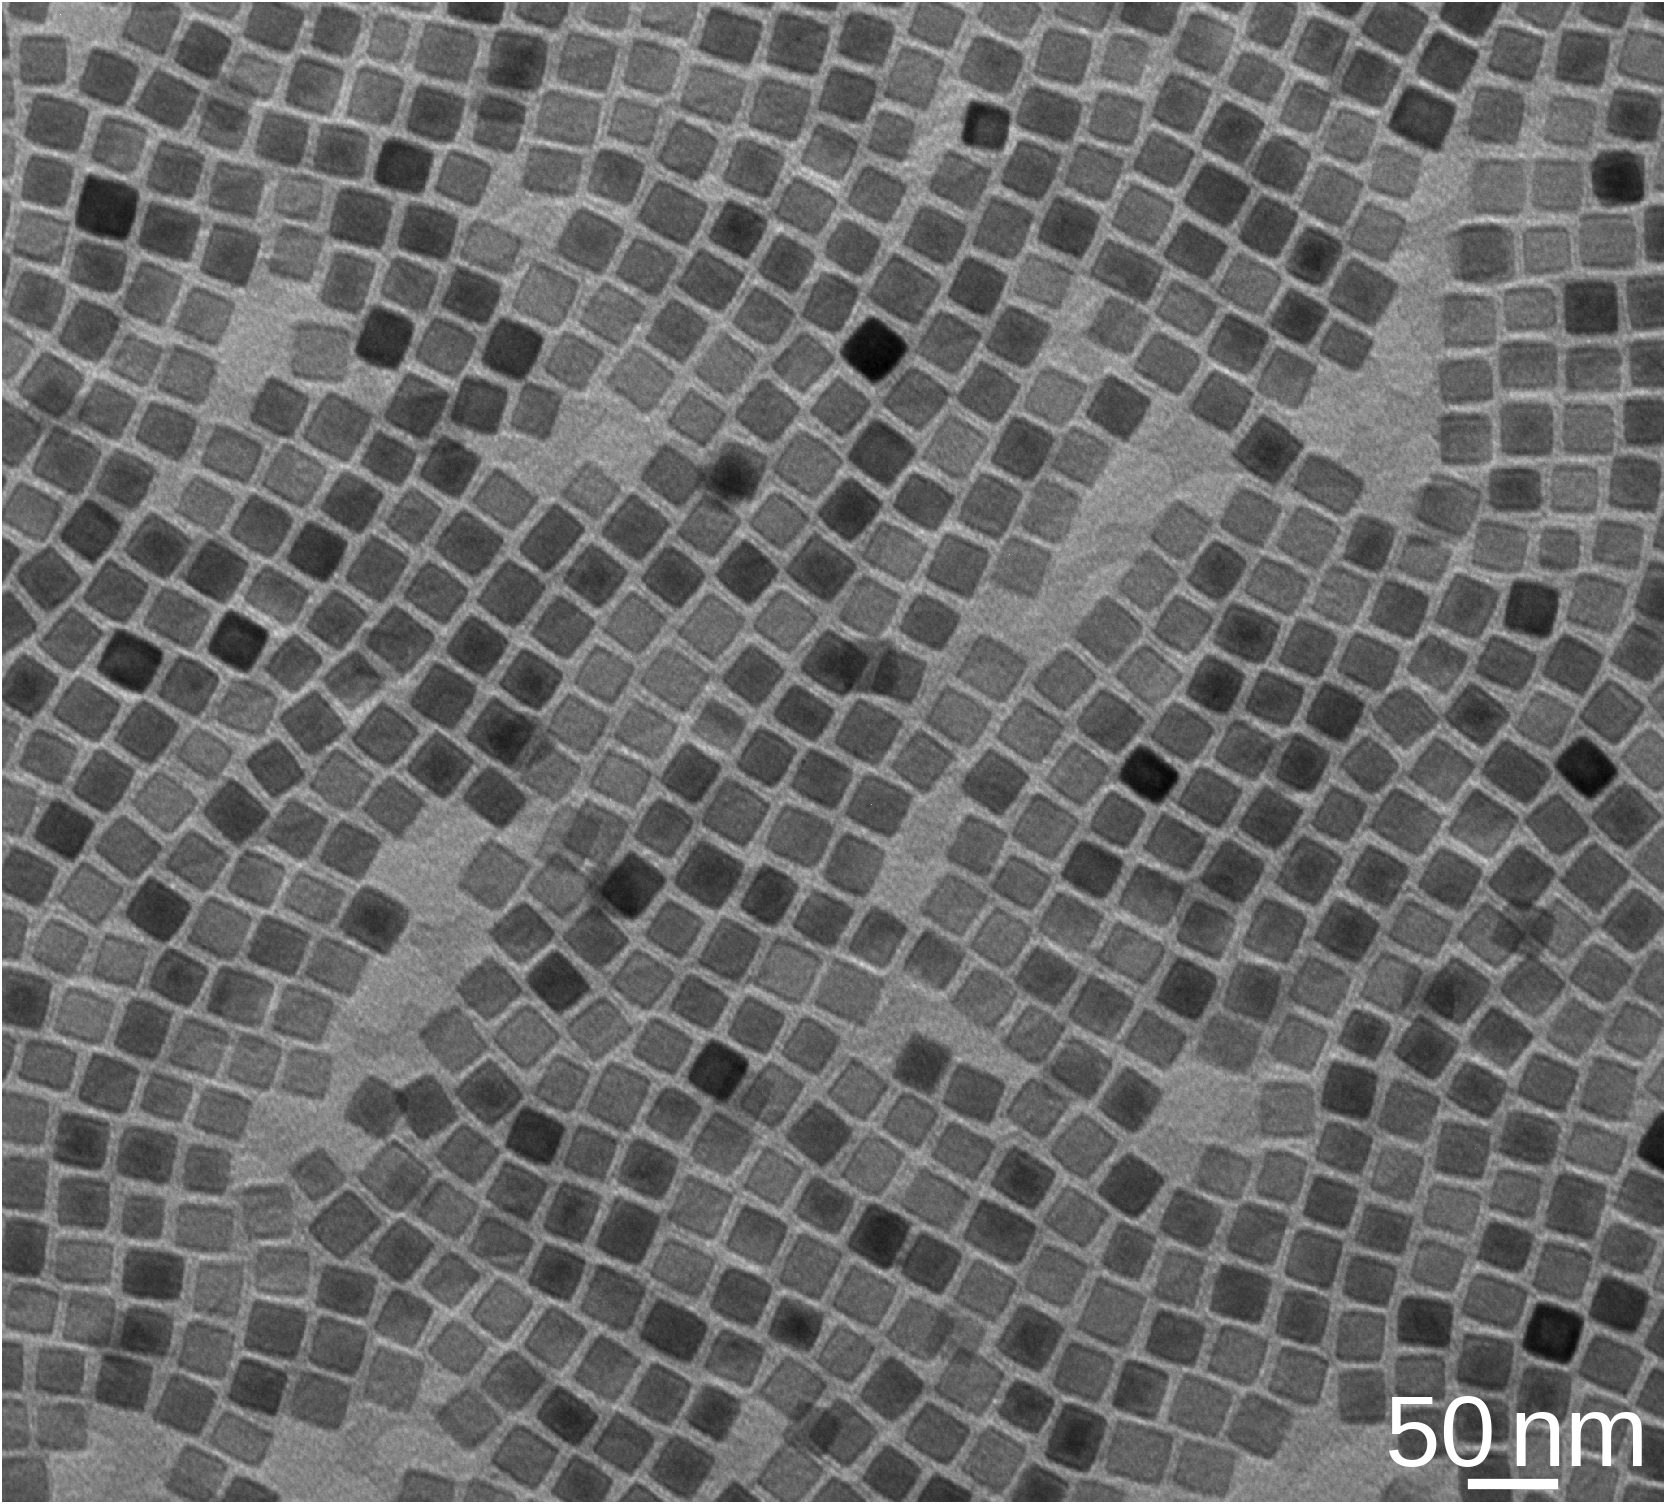
\includegraphics{monolayers_TEM_Ol_CoFe_C}
      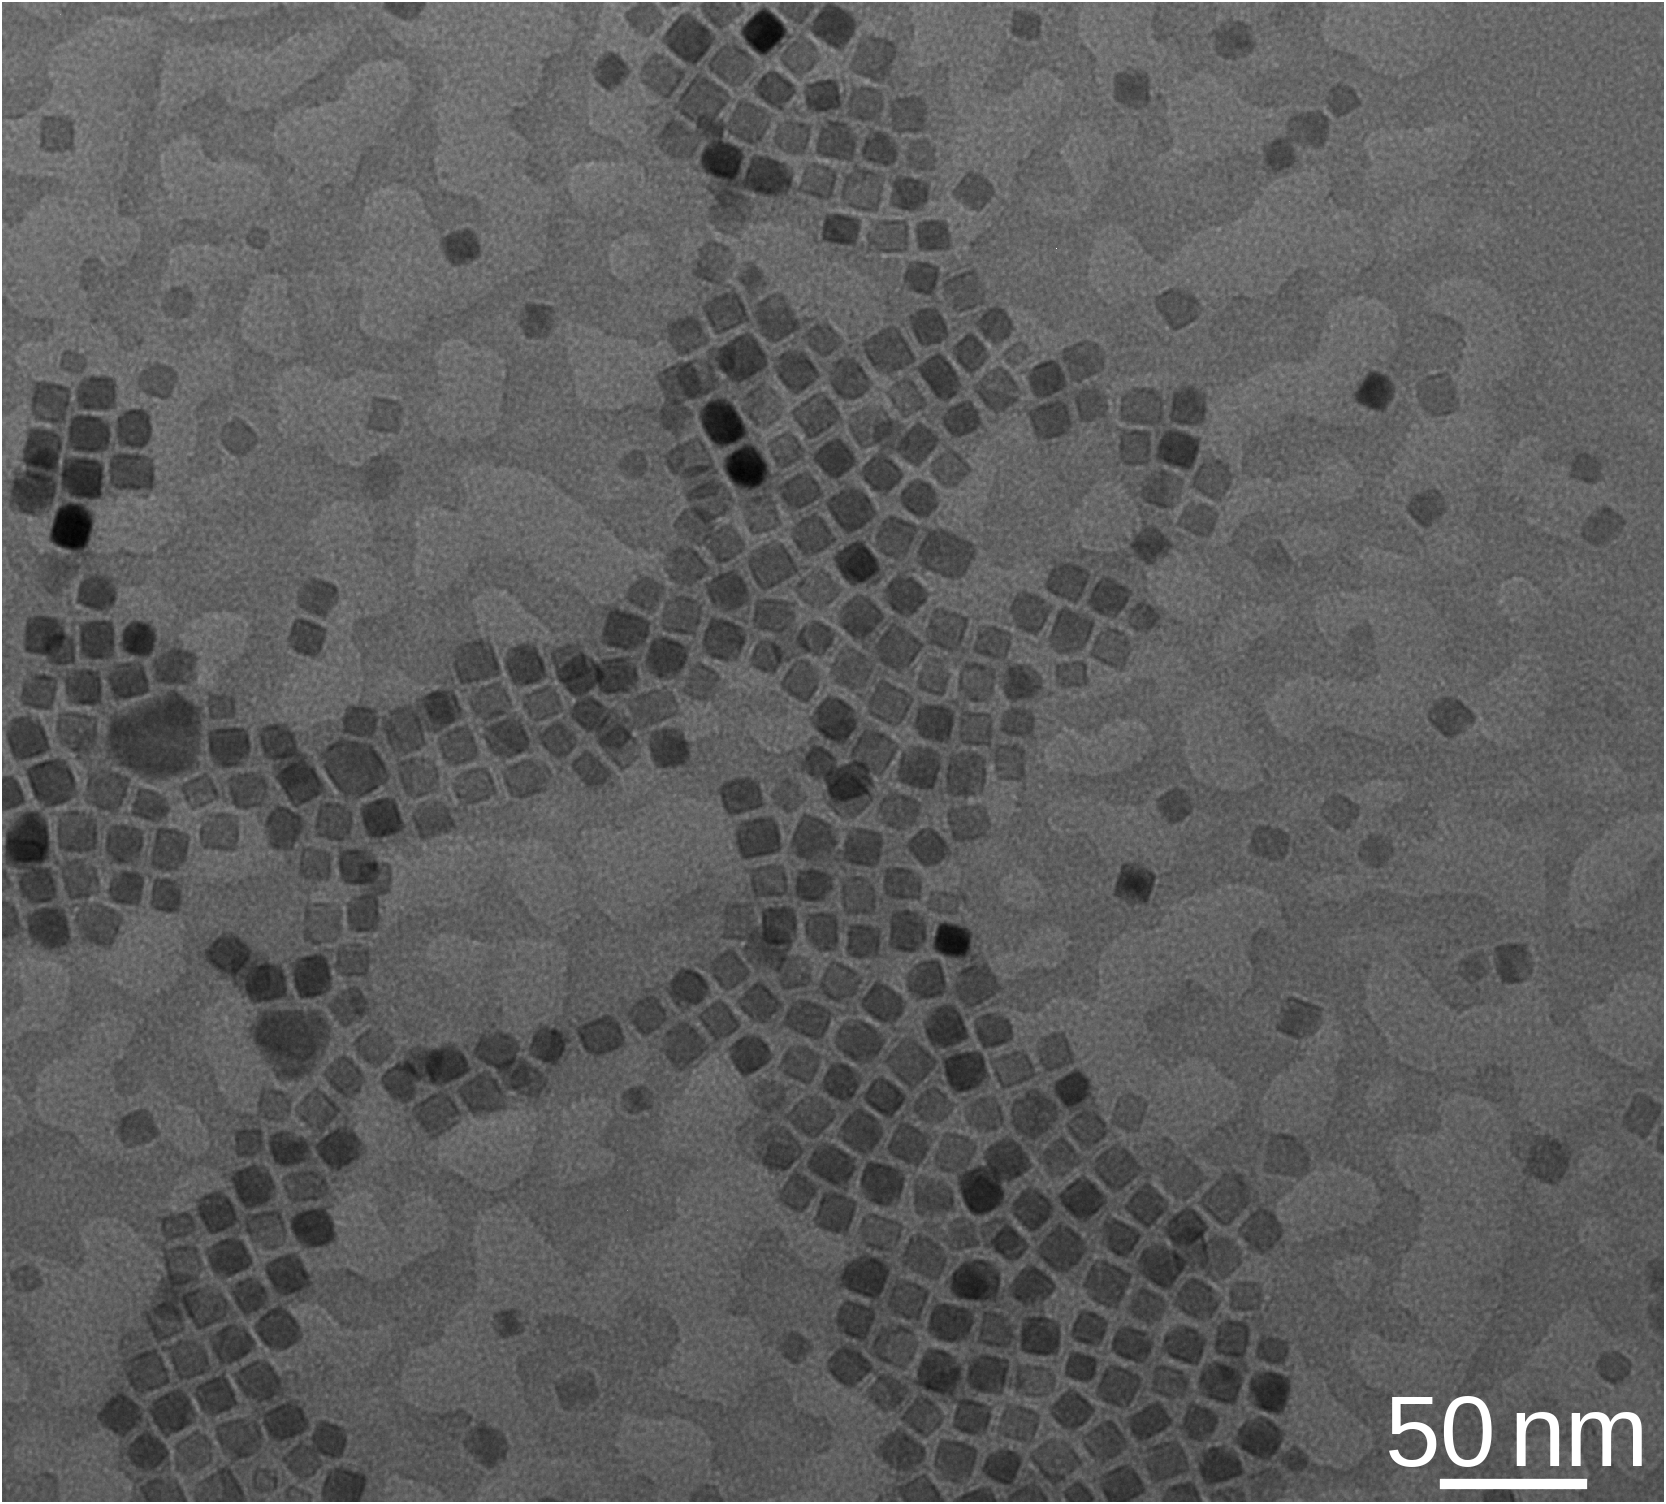
\includegraphics{monolayers_TEM_Ac_CoFe_C}
      \caption{\label{fig:monolayers:nanoparticle:tem}Transmission electron microscopy images of cobalt ferrite nanocubes synthesized from oleates (left) and acetylacetonates (right).}
    \end{figure}

    A quantitative evaluation of the transmission electron microscopy images in \reffig{fig:monolayers:nanoparticle:tem:fig:monolayers:nanoparticle:tem:edgelengths}
    \begin{figure}[tb]
      \centering
      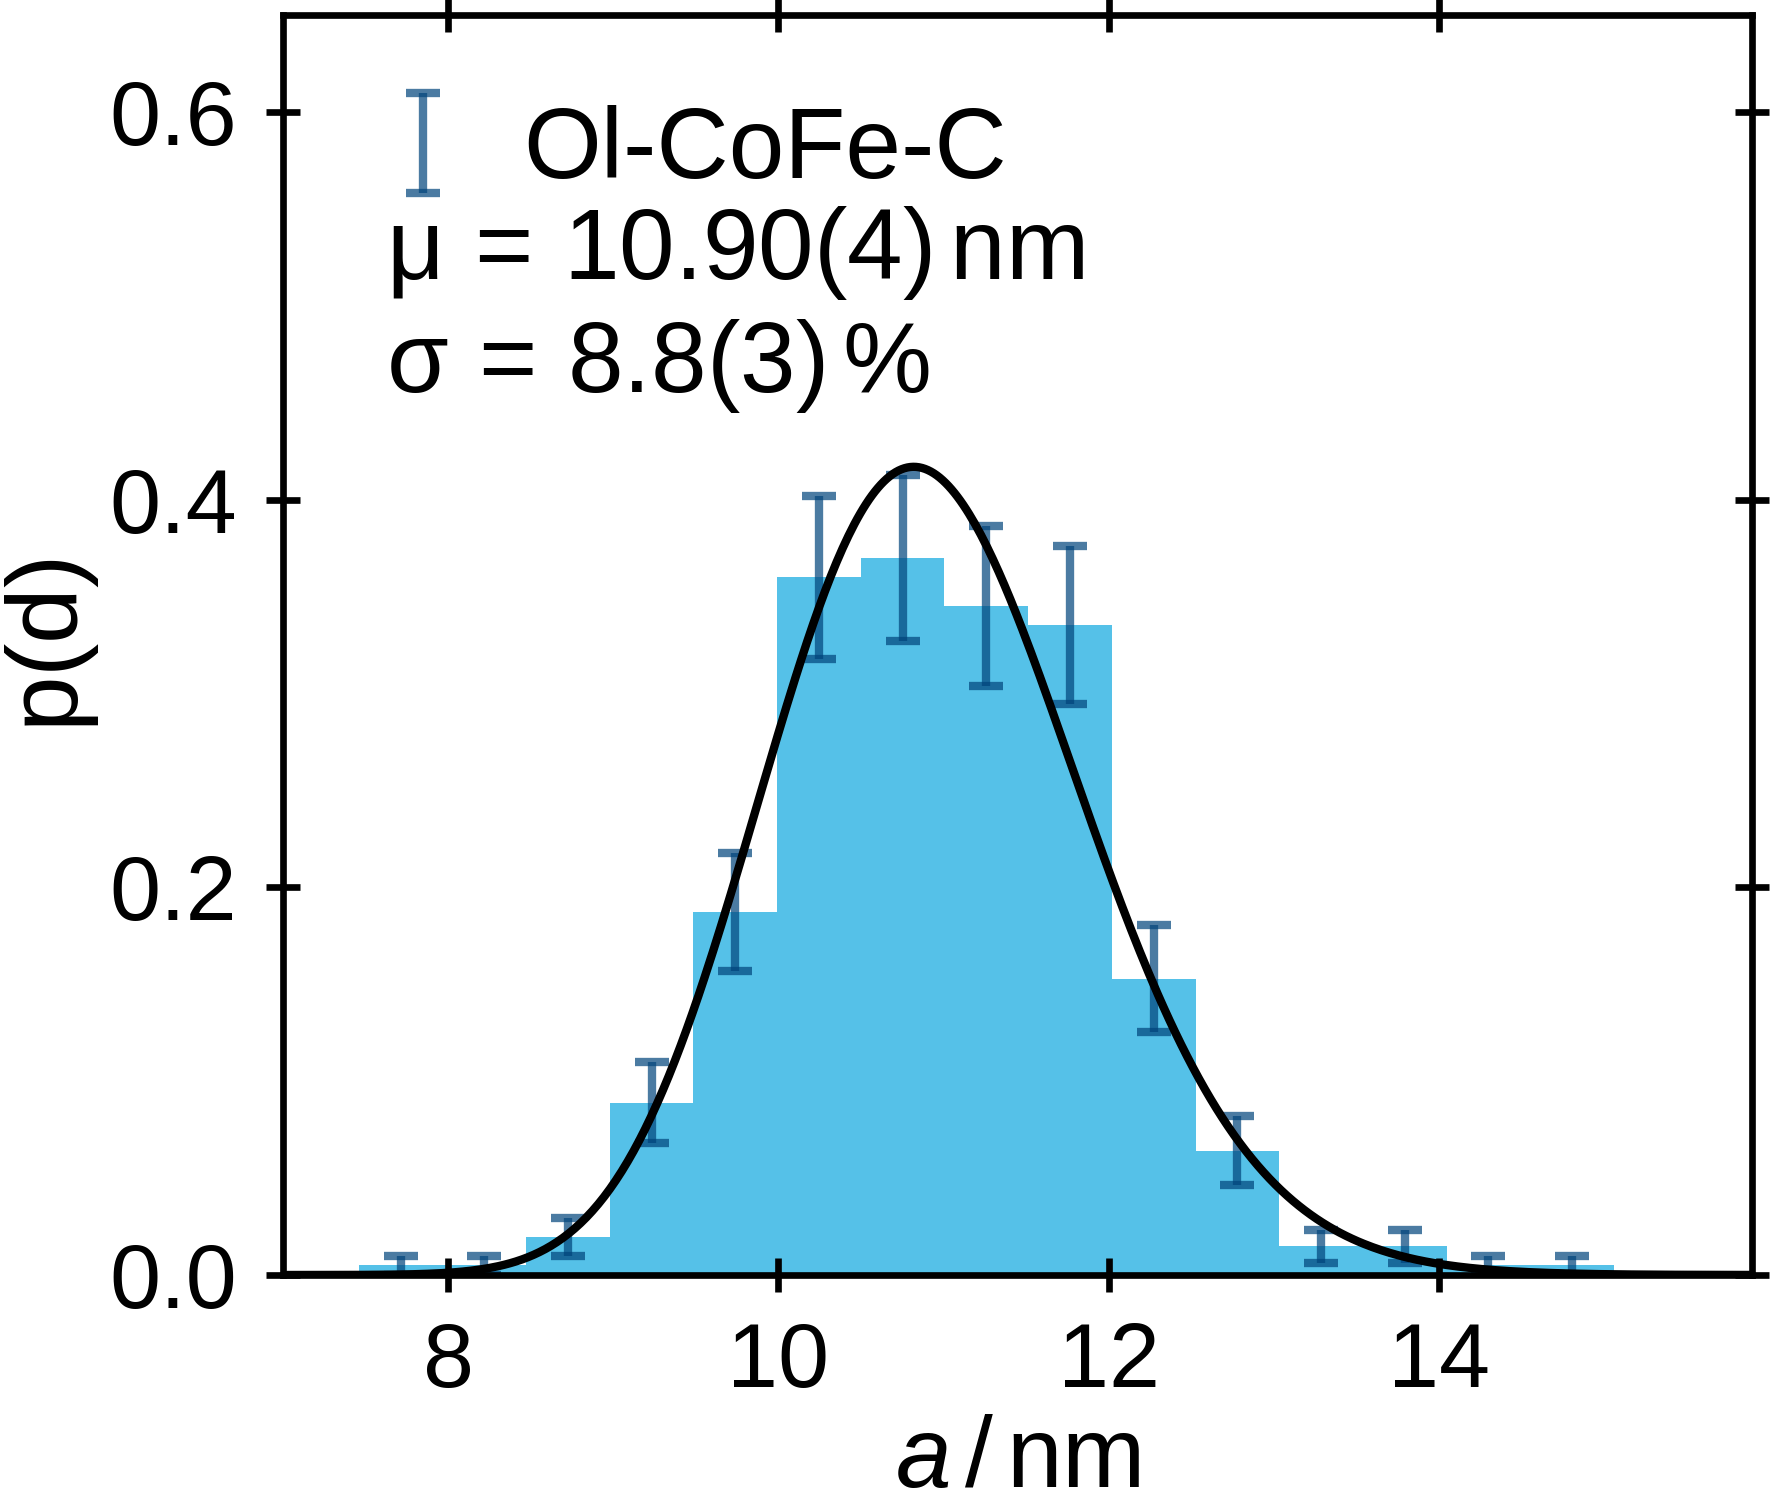
\includegraphics{monolayers_TEM_Ol_CoFe_C_sizeDist}
      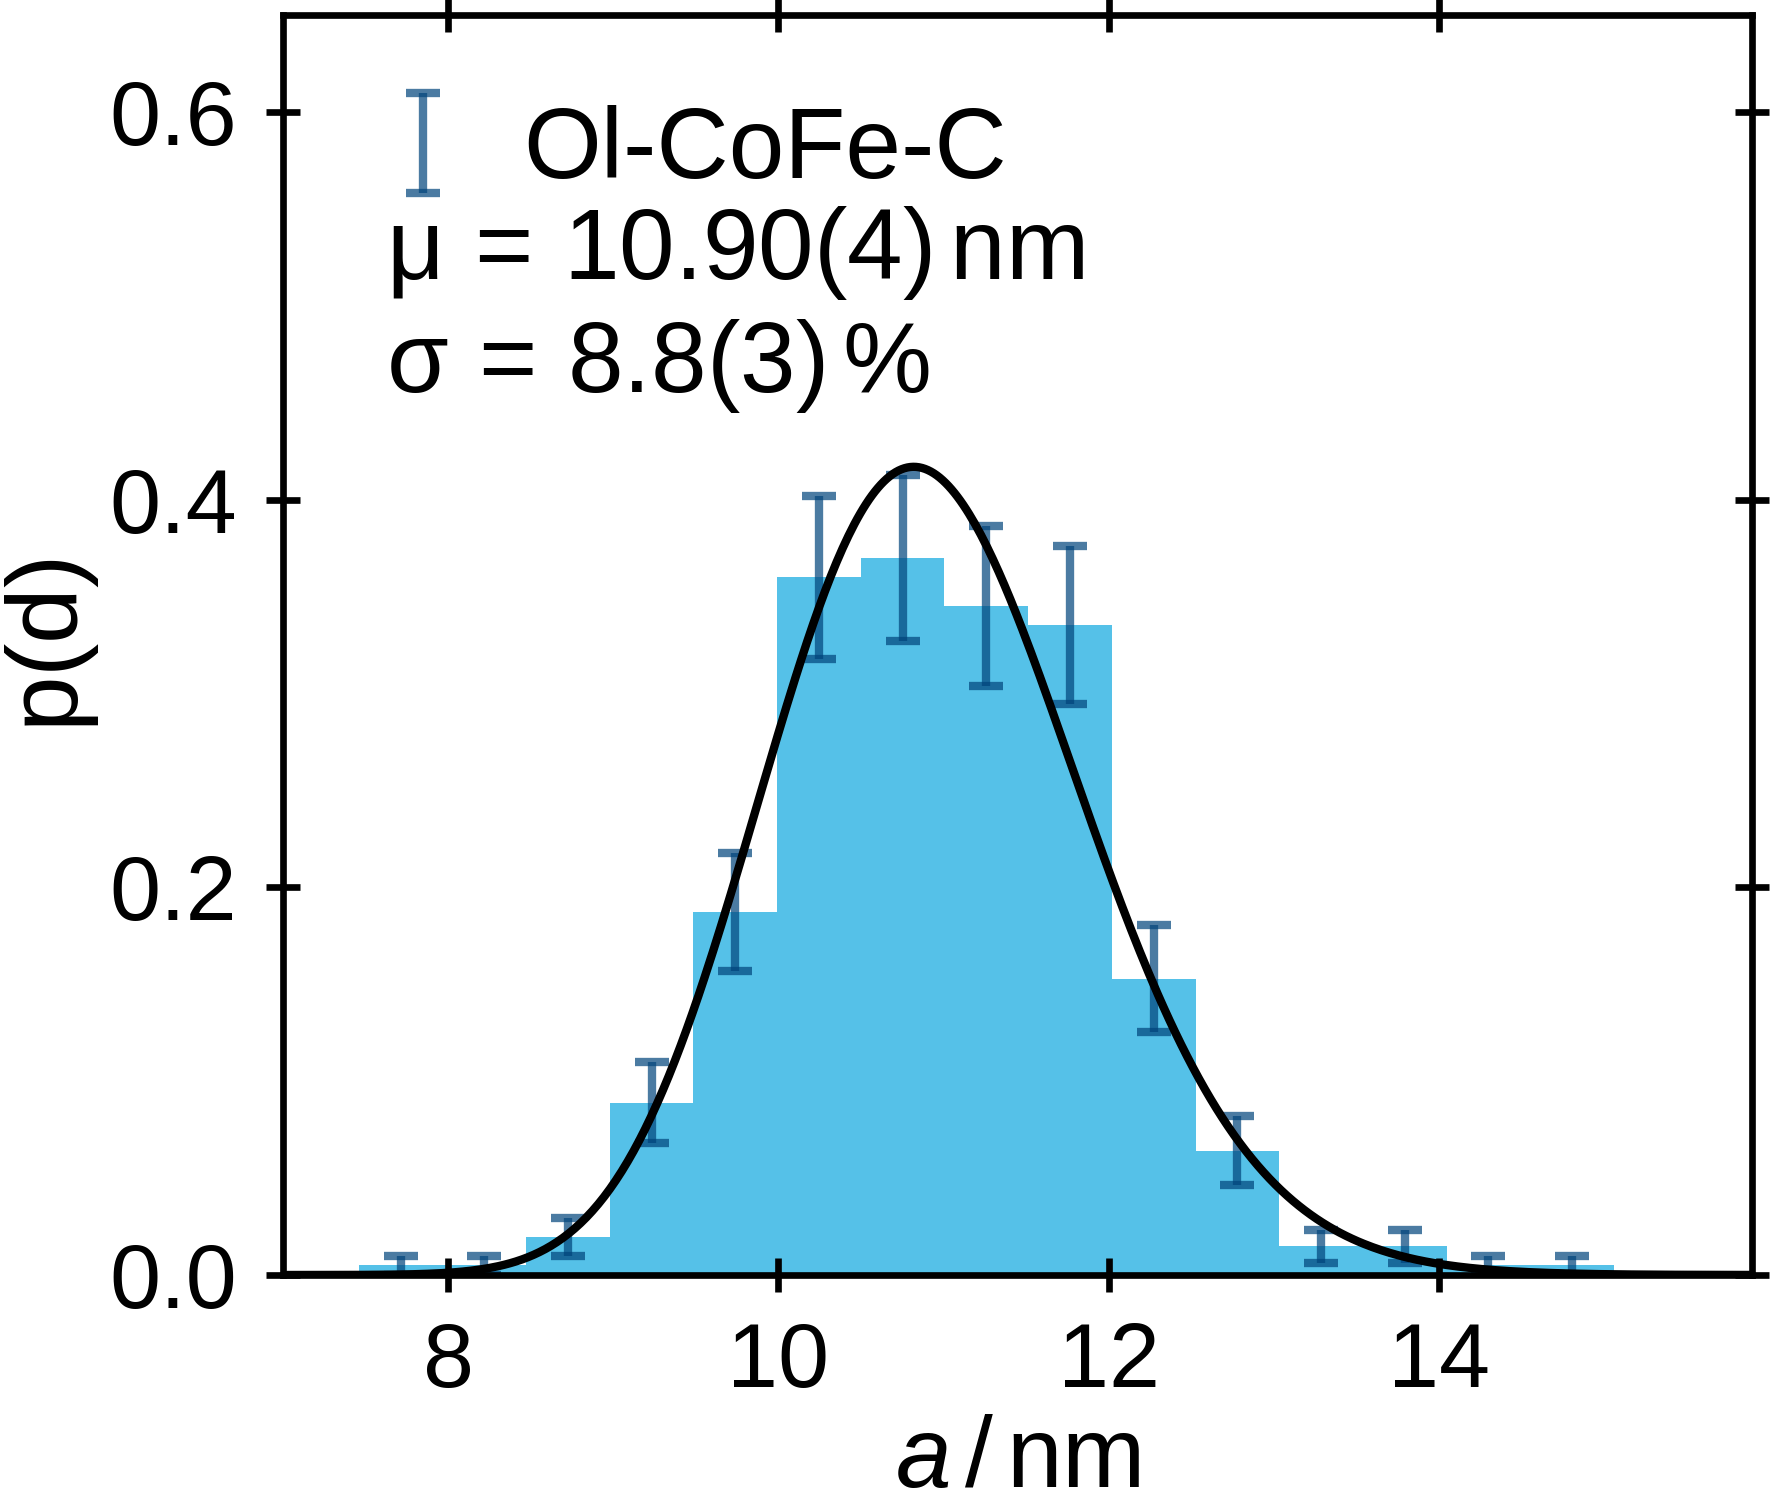
\includegraphics{monolayers_TEM_Ol_CoFe_C_sizeDist}
      \caption{\label{fig:monolayers:nanoparticle:tem:edgelengths}Edge length size distribution of the  of the nanocubes synthesized from oleates (left) and acetylacetonates (right).}
    \end{figure}

    \begin{figure}[tb]
      \centering
      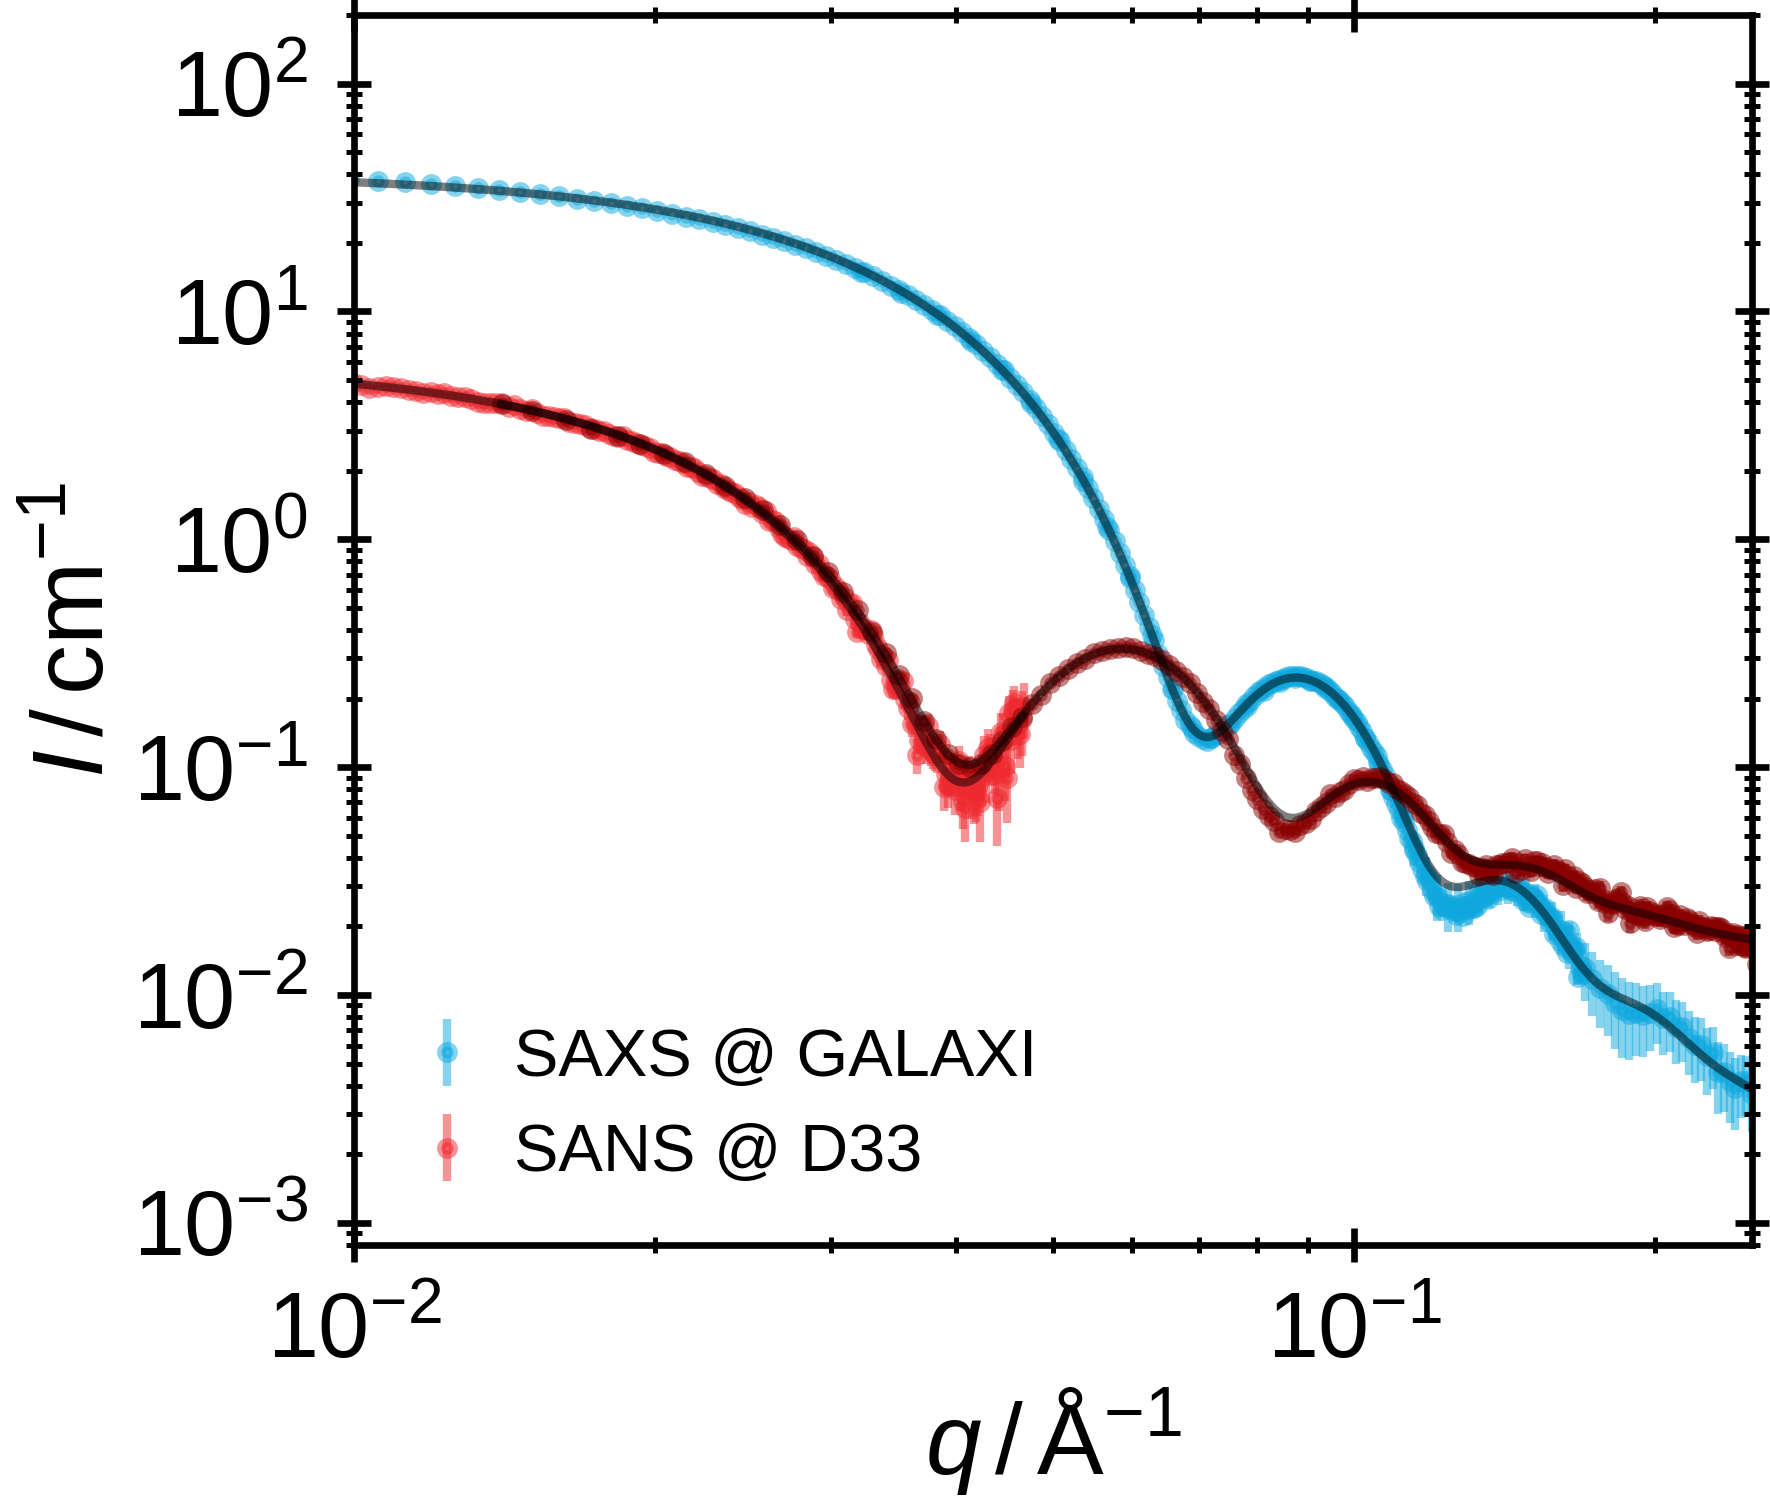
\includegraphics{monolayers_SAS_Ol_CoFe_C_SASFit}
      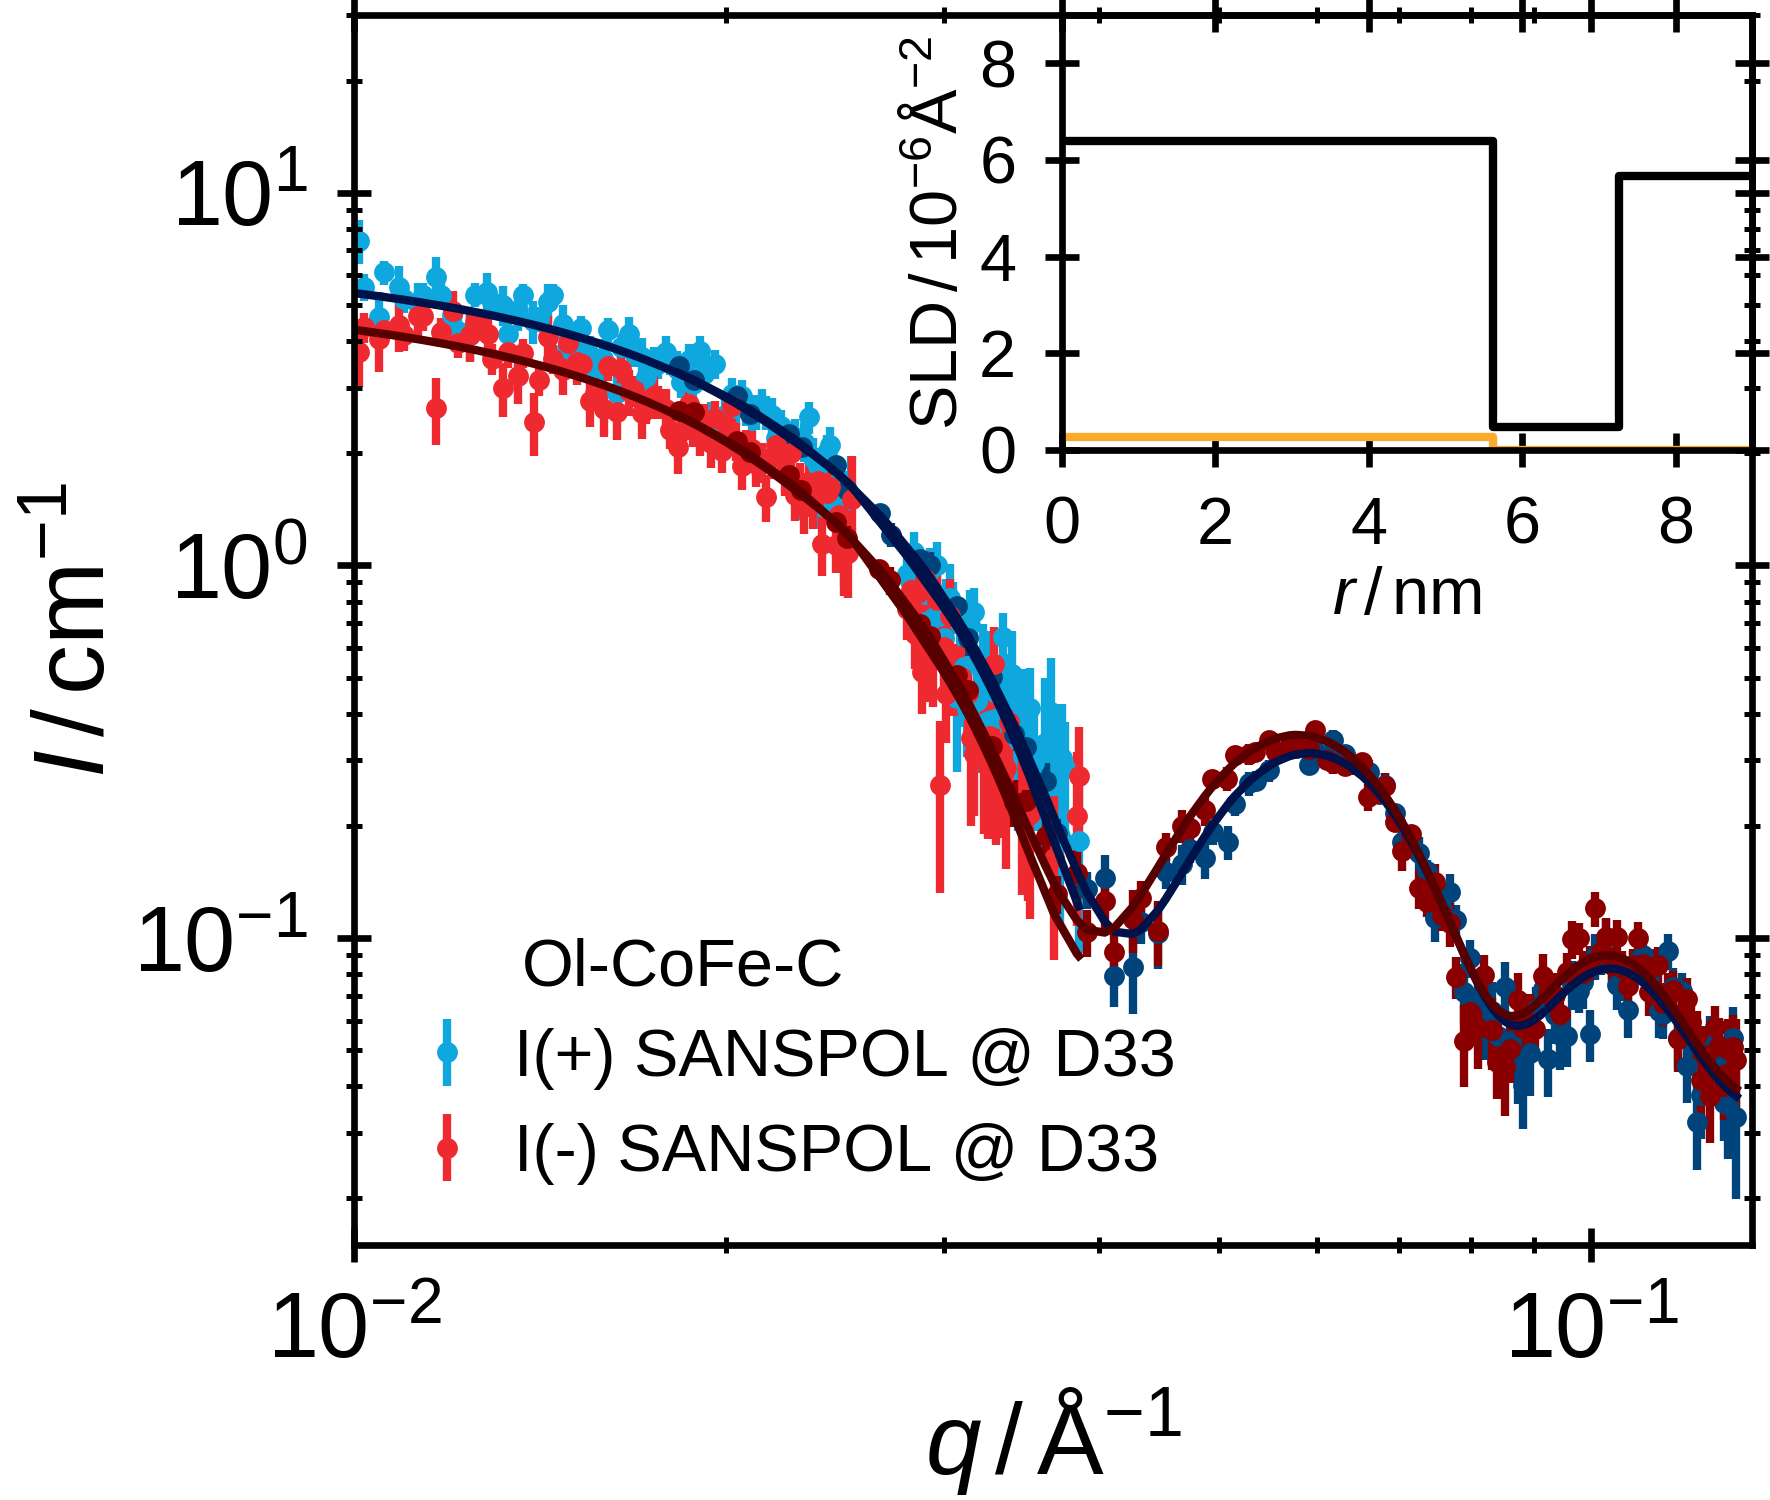
\includegraphics{monolayers_SAS_Ol_CoFe_C_SANSPOLFit}
      \caption{\label{fig:monolayers:nanoparticle:sas}Small-angle x-ray and neutron scattering for IOS-11 (left) and IOS-7 (right). The x-ray and neutron datasets are fitted simultaneously to a spherical core-shell model to estimate the average size of the particle size and surfactant shell.}
    \end{figure}
\end{document}